\section{Weiterentwicklung}

In der zweiten Phase des Projekts soll die Funktionalität des KSM erweitert werden. Besonderes Augenmerk liegt hierbei auf der Verbesserung der Anzeige, welche Knoten im aktiven/passiven, oder kritischen Bereich liegen. Diese Anzeige wird intern auch Sum-Chart genannt. Hier wurde bereits in einer der letzten Studienarbeiten von Frau Klein angefangen, es dem Benutzer zu ermöglichen, Bereiche zu definieren und zu markieren \cite{bib:klein}. Bereiche waren in diesem Fall Ellipsen, die vom Benutzer aufgezogen wurden. Je größer diese wurden, desto transparenter wurde die Füllfarbe. Die Abbildung \ref{ellipse} zeigt den letzten Stand dieser Implementierung.
\begin{figure}[h]
	\centering
	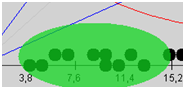
\includegraphics[width=0.4\textwidth]{pictures/ellipse.png}
	\caption{Bereichsmarkierung nach Klein \cite{bib:klein}}
	\label{ellipse}
\end{figure}

Nach Evaluation dieser Implementierung kam Herr Professor Schubert zu dem Schluss, dass Ellipsen auf der einen Seite zu unflexibel sind, um einen Bereich adäquat ausbilden zu können. Auf der anderen Seite jedoch auf keinerlei Begrenzungen, wie zum Beispiel aktiv, passiv Geraden  Rücksicht nehmen. Dazu wurde die Füllfarbe trotz Transparenz teilweise als zu deckend empfunden.

\subsection{Anforderungen}

Die neuen Anforderungen an eine Bereichsmarkierung lauteten nach diesen Erkenntnissen wie folgt:
\begin{itemize}
  \item Der Benutzer muss in der Lage sein, einen Bereich mittels Eckpunkten definieren zu können
  \item Es dürfen beliebig viele Eckpunkte sein
  \item Die Eckpunkte dürfen nur auf Bereits vorhandenen Linien laufen:
  \begin{itemize}
    \item X-Achse
    \item Y-Achse
    \item Q-Achsen zur Abgrenzung der aktiven/passiven Bereiche, sowie Q = 1 als Mitte
    \item Hyperbeln zur Markierung des stabilen/kritischen Bereichs
  \end{itemize}
  \item Punkte (Knoten des System Graphen), die innerhalb des markierten Bereichs liegen, müssen aufgelistet werden
  \item Die Füllfarbe des Bereichs soll transparenter sein, als bisher
\end{itemize}

Dazu wurde noch von den Projektmitgliedern entschieden, dass erstellte Bereiche benannt werden sollen. Dieser Name soll innerhalb des Bereichs sichtbar sein.

\subsection{Ergebnis}

Die gestellten Anforderungen wurden vollständig umgesetzt. Der Benutzer kann nun durch setzen mehrerer Eckpunkte, die sich auf den vorgegebenen Linien befinden ein Polygon definieren.

Damit der Benutzer immer weiß, wo der nächste Eckpunkt gesetzt werden würde, wurde ein roter Punkt implementiert, der sich nur auf den erlaubten Linien bewegt und so den nächsten Eckpunkt markiert (Abbildung \ref{roterPunkt}).
\begin{figure}[h]
	\centering
	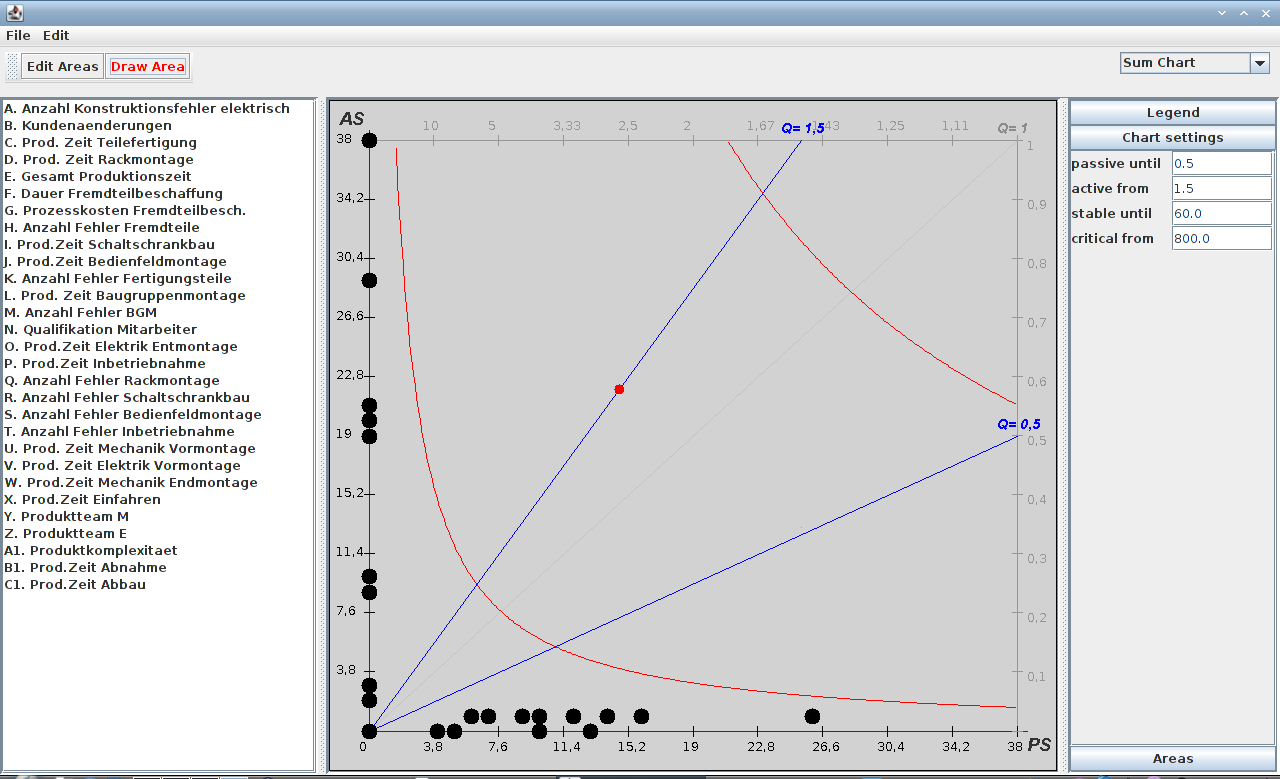
\includegraphics[width=0.7\textwidth]{pictures/roter-punkt.png}
	\caption{roter Punkt}
	\label{roterPunkt}
\end{figure}

Mittels Klick wird der Punkt gespeichert und ein vorläufiges Polygon gezeichnet. Will der Benutzer die Eingabe beenden, kann er das Polygon mit einem Doppelklick abschließen. Anschließend wird einen Auswahldialog präsentiert, ob das Polygon übernommen, oder verworfen werden soll.
Abbildung \ref{menü} zeigt ein abgeschlossenes Polygon und das Auswahlmenü.
\begin{figure}[h]
	\centering
	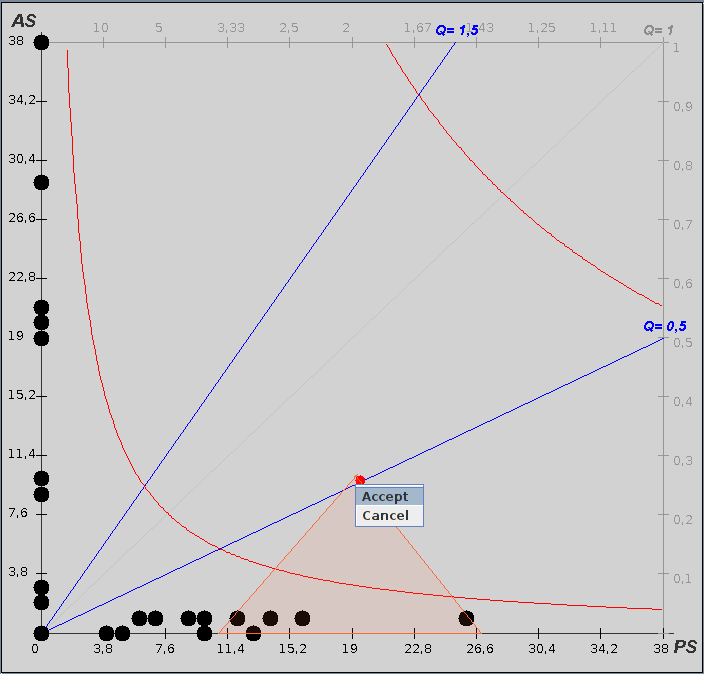
\includegraphics[width=0.7\textwidth]{pictures/menu.png}
	\caption{abgeschlossenes Polygon mit Auswahldialog}
	\label{menü}
\end{figure}

Nachdem ein Polygon akzeptiert und benannt wurde, wird ermittelt das Programm, welche Knoten sich innerhalb dieses Polygons befinden und listet diese in einer Baumstruktur auf. Diese Auflistungen können im rechten Panel unter dem Eintrag ``Areas'' gefunden werden. Abbildung \ref{baum} zeigt diese Auflistung für das Polygon ``Beispiel''.
\begin{figure}[h]
	\centering
	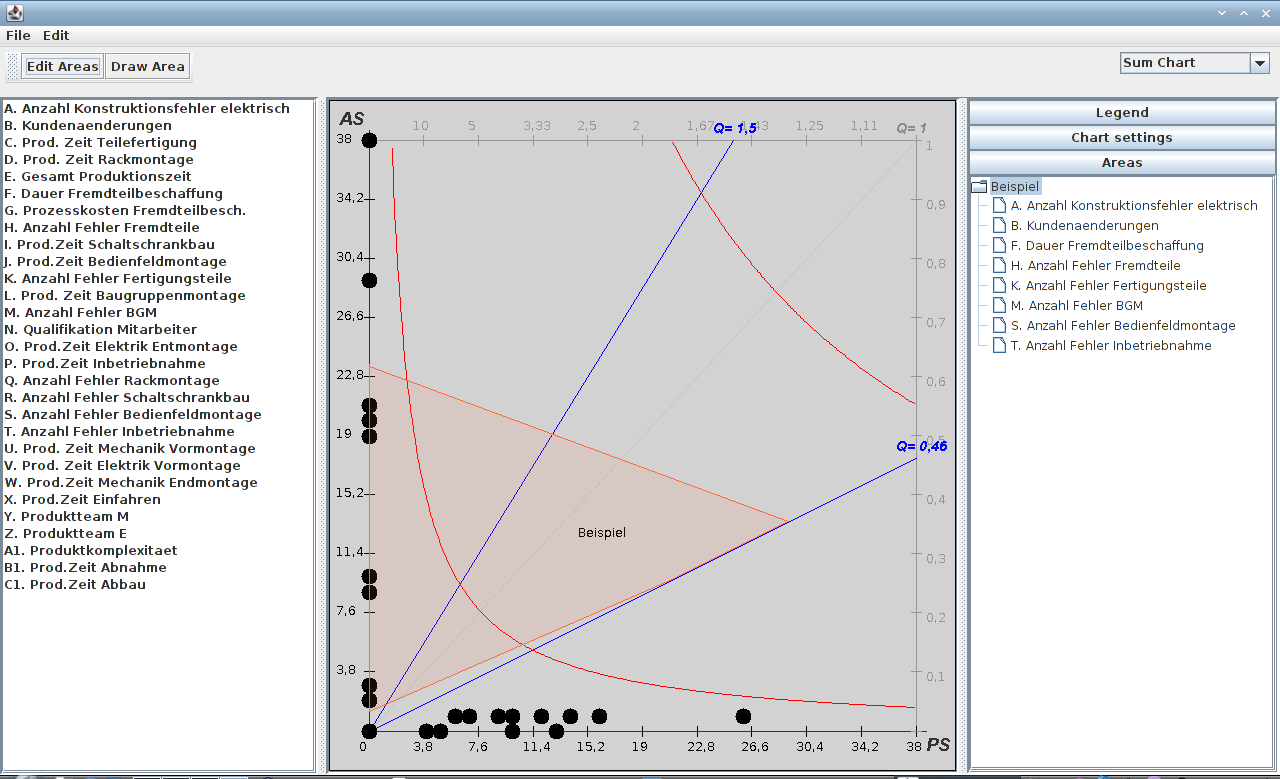
\includegraphics[width=1\textwidth]{pictures/baum.png}
	\caption{Baumdarstellung der Knoten innerhalb eines Polygons}
	\label{baum}
\end{figure}

Die Anforderung der zu geringen Transparenz wurde etwas anders gelöst, als anfangs geplant. Die ursprüngliche Implementierung von Frau Klein sah vor, dass die Transparenz mit der Größe der Fläche zunimmt. Dieser Umstand führte in der neuen Implementierung dazu, dass obwohl der Transparenzwert erhöht wurde, kleine Flächen immer noch viel zu deckend waren. Große Flächen jedoch kaum noch sichtbar waren. Deswegen wurde die Kopplung der Transparenz mit der Fläche aufgehoben und stattdessen eine starke Transparenz der Füllfarbe definiert und die Fläche zudem mit einer deckenden Umrandung versehen. Dies ermöglicht eine gute Sichtbarkeit der Knoten und Werte innerhalb des Polygons, bei gleichzeitiger guter Sichtbarkeit des Polygons selbst, wie auf den Abbildungen \ref{baum} und \ref{menü} zu sehen ist.



\subsection{Implementierung}
